
\section{Results}

\subsection{The COMBINE archive}
During my work I kept the COMBINE archive in a GIT repository for version control.
The latest version of the archive can be found at GitHub\footnote{\href{https://github.com/SemsProject/CombineArchiveShowCase}{github.com/SemsProject/CombineArchiveShowCase}}, the latest archive can be downloaded from our website\footnote{\href{http://scripts.sems.uni-rostock.de/getshowcase.php}{scripts.sems.uni-rostock.de/getshowcase.php}}.
At the time of writing this report\footnote{latest git commit: 2e946ce1adfd05d16350c30176e29546301603a2 -- 2015-06-11}, the archive consists of 25 files organized in four directories (cmp. Section~\ref{sec:extendingarchive}), including the \texttt{manifest.xml} and \texttt{metadata.rdf} (the skeleton of the archive, see Section~\ref{sec:intro}) and a \texttt{README.md} file for the GitHub repository.
The manifest listing all ingredients of the COMBINE archive is attached in Section~\ref{sec:manifest}.

The archive basically consists of 4 modules: (i) the publication stored in the \texttt{documentation/} directory, (ii) the model of the biological system encoded in standardised formats stored in the \texttt{model/} directory, (iii) the simulation description encoded in \sedml stored in the \texttt{experiment/} directory, (iv) the simulation results in form of graphs stored in the \texttt{result/} directory.
The files in these directories were either retrieved from other websites (publication, SBML model, CellML model) or generated especially for this archive (\sedml scripts, simulation results, SBGN map).
The goal of this archive is to encode a reproducible simulation study.
Figure~\ref{fig:sim:results} has shown that the developed study is able to reproduce graphs shown in the corresponding publication.

\subsection{Reproducible Simulation Study}

\begin{figure}
\begin{center}
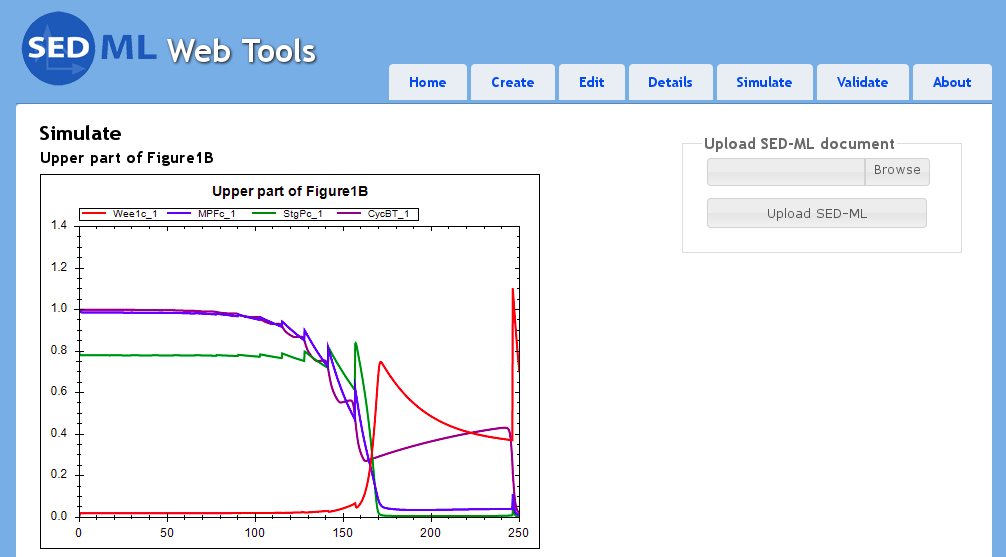
\includegraphics[width=.78\textwidth]{img/swt-reproduced-cropped.png}
\end{center}
\caption{\textbf{Reproduced Results.} The results were reproduced by uploading the COMBINE archive to the \sedml Web Tools.}
\label{fig:swt-repro}
\end{figure}

The developed study can easily be reproduced using the SWT, which provides a neat API.
As the archive can be obtained from \href{http://scripts.sems.uni-rostock.de/getshowcase.php}{scripts.sems.uni-rostock.de/getshowcase.php} you can import the archive by passing the link to the archive as the \texttt{url} parameter to the SWT.
In other words, open the following URL in your browser:

% \begin{center}
{\href{http://bqfbergmann.dyndns.org/SED-ML_Web_Tools/Home/SimulateUrl?url=http://scripts.sems.uni-rostock.de/getshowcase.php}{\texttt{{\tiny{bqfbergmann.dyndns.org/SED-ML\_Web\_Tools/Home/}}{\scriptsize{SimulateUrl?url=http://scripts.sems.uni-rostock.de/getshowcase.php}}}}}
% \end{center}

The SWT will immediately present you the results as shown in Figure~\ref{fig:swt-repro}.

The SWT API also allows you to run the simulation encoded in the demo archive without visiting a website.
You can simply send the archive using an HTTP POST request and obtain the simulation results, which are again encoded in a COMBINE archive:

\begin{mdframed}[style=mddefault,frametitle={Obtain the simulation results using the API of the \sedml Web Tolls}]
\begin{minted}[linenos,breaklines=true,numbersep=5pt,tabsize=2,xleftmargin=-7pt,fontsize=\footnotesize]{bash}
wget -O demoarchive.omex http://scripts.sems.uni-rostock.de/getshowcase.php
curl -L -F file=@demoarchive.omex http://sysbioapps.dyndns.org/SED-ML_Web_Tools/Home/SimulatePostArchive > simulation-results.omex
\end{minted}
\end{mdframed}

You will then find the simulation results in the file \texttt{simulation-results.omex}.
To explore the obtained archive it can, for example, be uploaded to the CombineArchiveWeb application.

